\documentclass[../../Main.tex]{subfiles}

\begin{document}
\section{准备开发环境}
DDLC Mod模板是由GanstaKingofSA编写的一个方便开发Mod的模板。imgradeone对其进行了本土化。目前,DDLC Mod中文模板主要流行三个大版本:1.0版本,2.0版本(即Next分支)与4.0版本(即Future分支)。
\begin{itemize}
    \item 1.0 版本仅支持 Ren'Py 6,且没有什么特别功能;
    \item 2.0 版本增加支持了 Ren'Py 7、Android 移植等功能;
    \item 4.0 版本增加支持了 Ren'Py 8 与 Python 3,增加额外屏幕(Extra Screen)功能等,但稳定性存疑。
\end{itemize}

本书将使用 2.0 版本进行讲解。

\subsection{下载DDLC Mod中文模版}
\label{2.1.1}

\begin{figure}[htb]
    \centering
    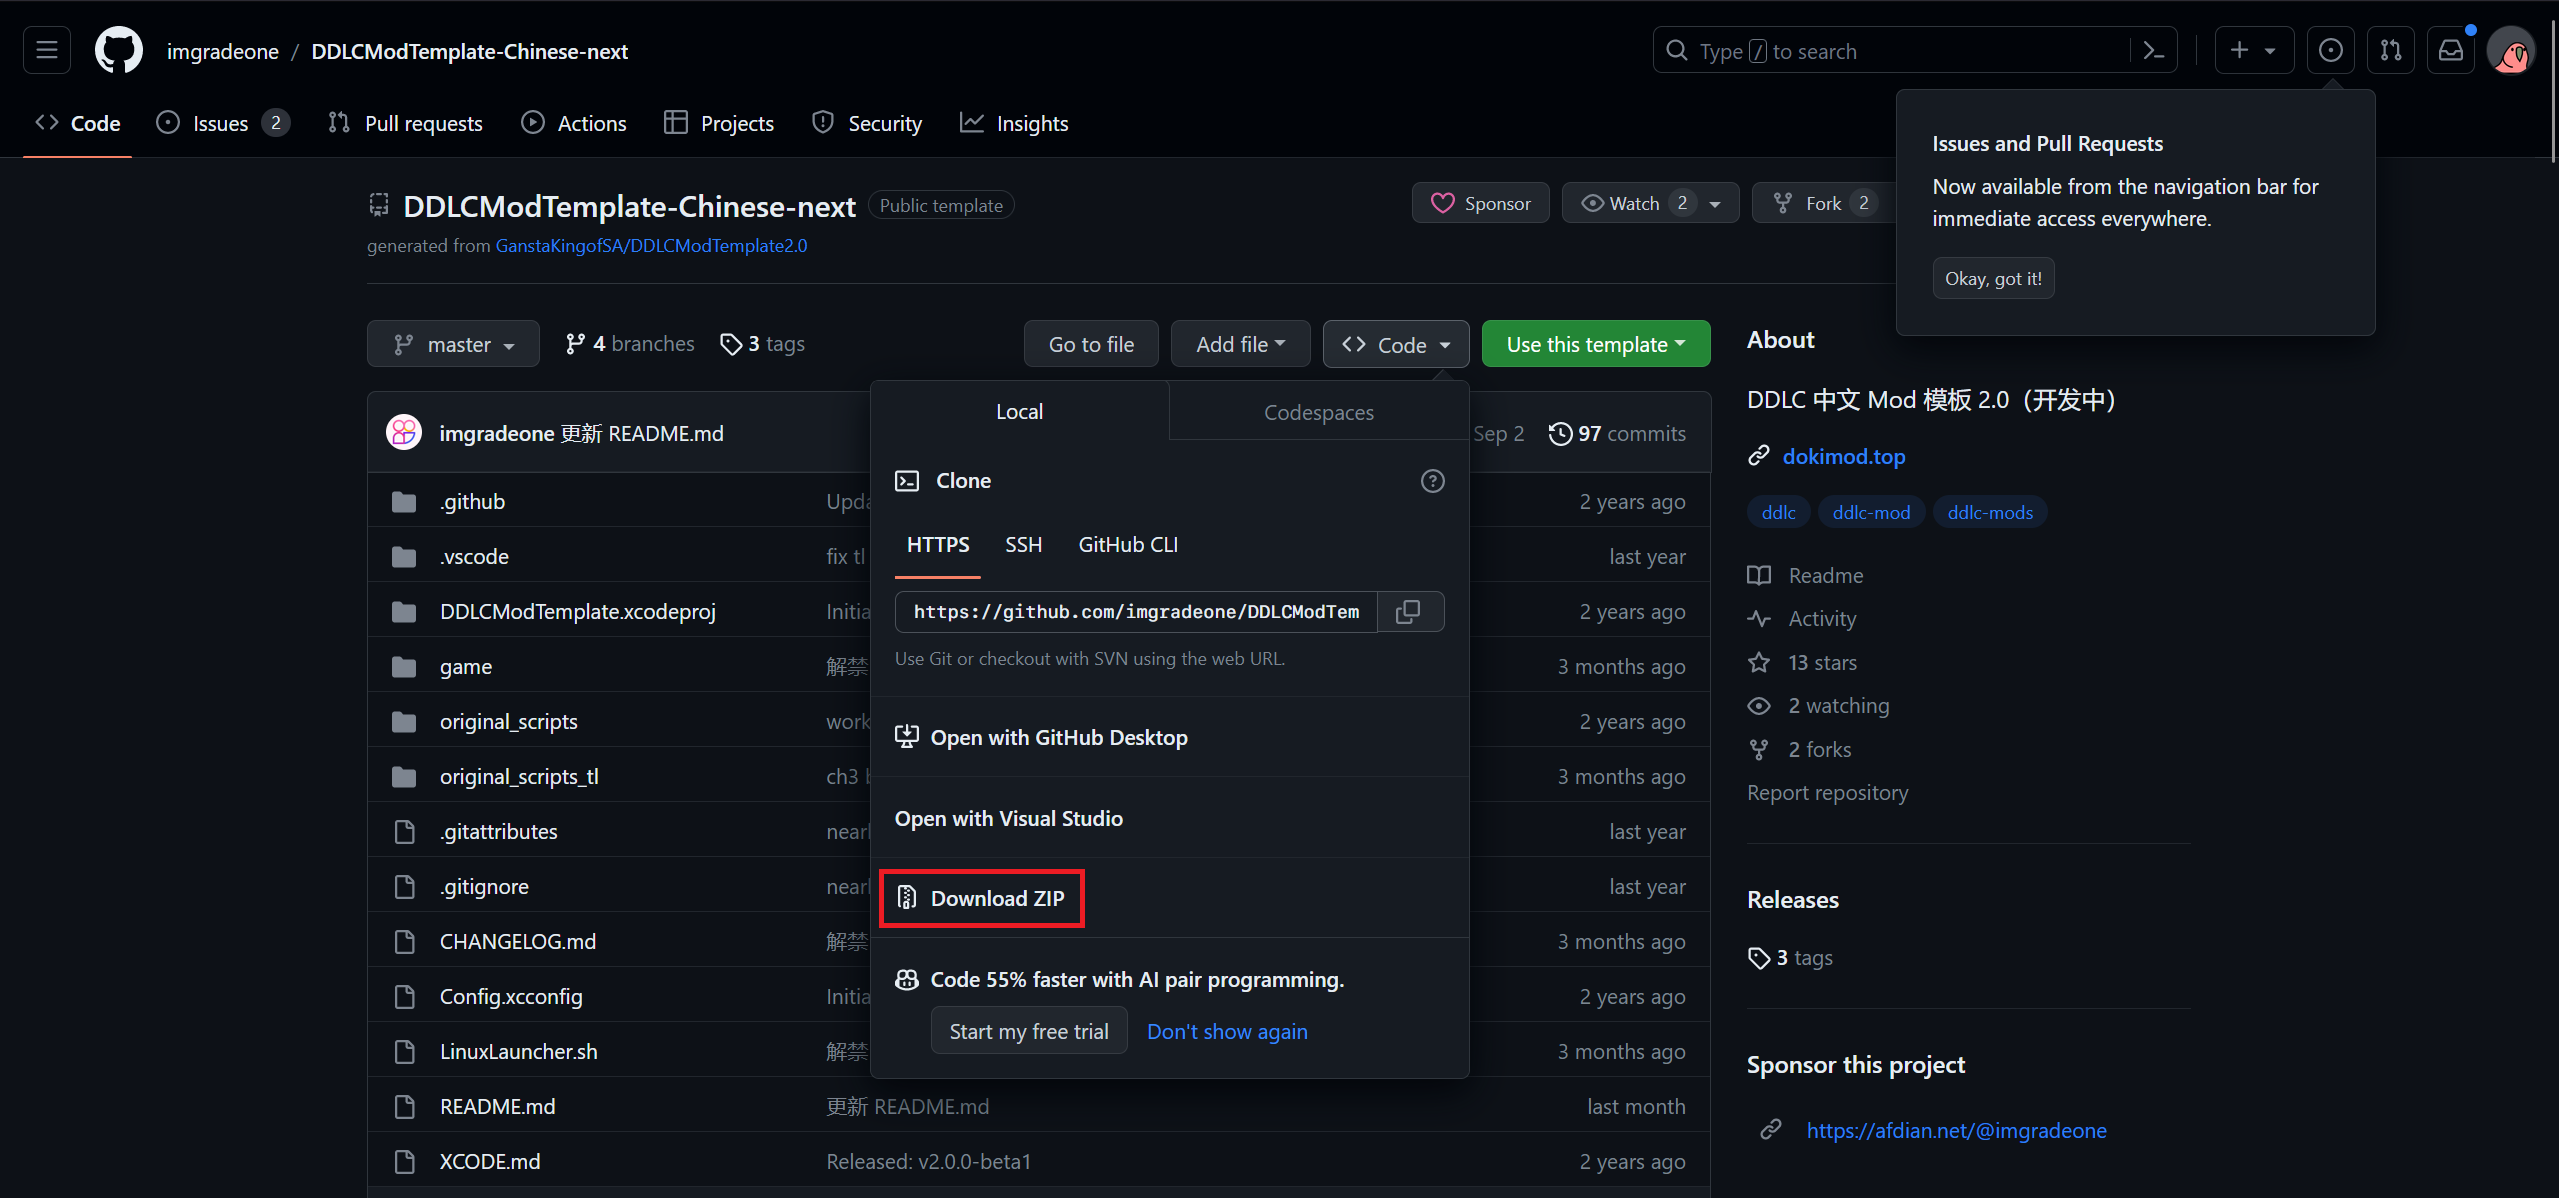
\includegraphics[scale=.15]{2.1/2.1.1}
    \caption{项目页面}
    \label{fig:2.1.1.1}
\end{figure}
使用任意浏览器打开\url{https://github.com/imgradeone/DDLCModTemplate-Chinese-next},将压缩包下载下来(如图\ref{fig:2.1.1.1}所示)。

下载完成后解压至在第\ref{sec:1.2.1}节中您下载的Ren'Py SDK的目录下。完成该步骤后,您的Ren'Py SDK中项目一栏应出现DDLCModTemplate-Chinese-next。

从 https://ddlc.moe/中下载原版DDLC,打开压缩包后将DDLC-1.1.1-pc/game/下的audio.rpa、images.rpa、fonts.rpa解压至Mod中文模板下的game/文件夹中。此时,Mod中文模板下的game/文件夹结构应如图\ref{fig:2.1.1.2}所示。

\begin{figure}[htbp]
    \centering
    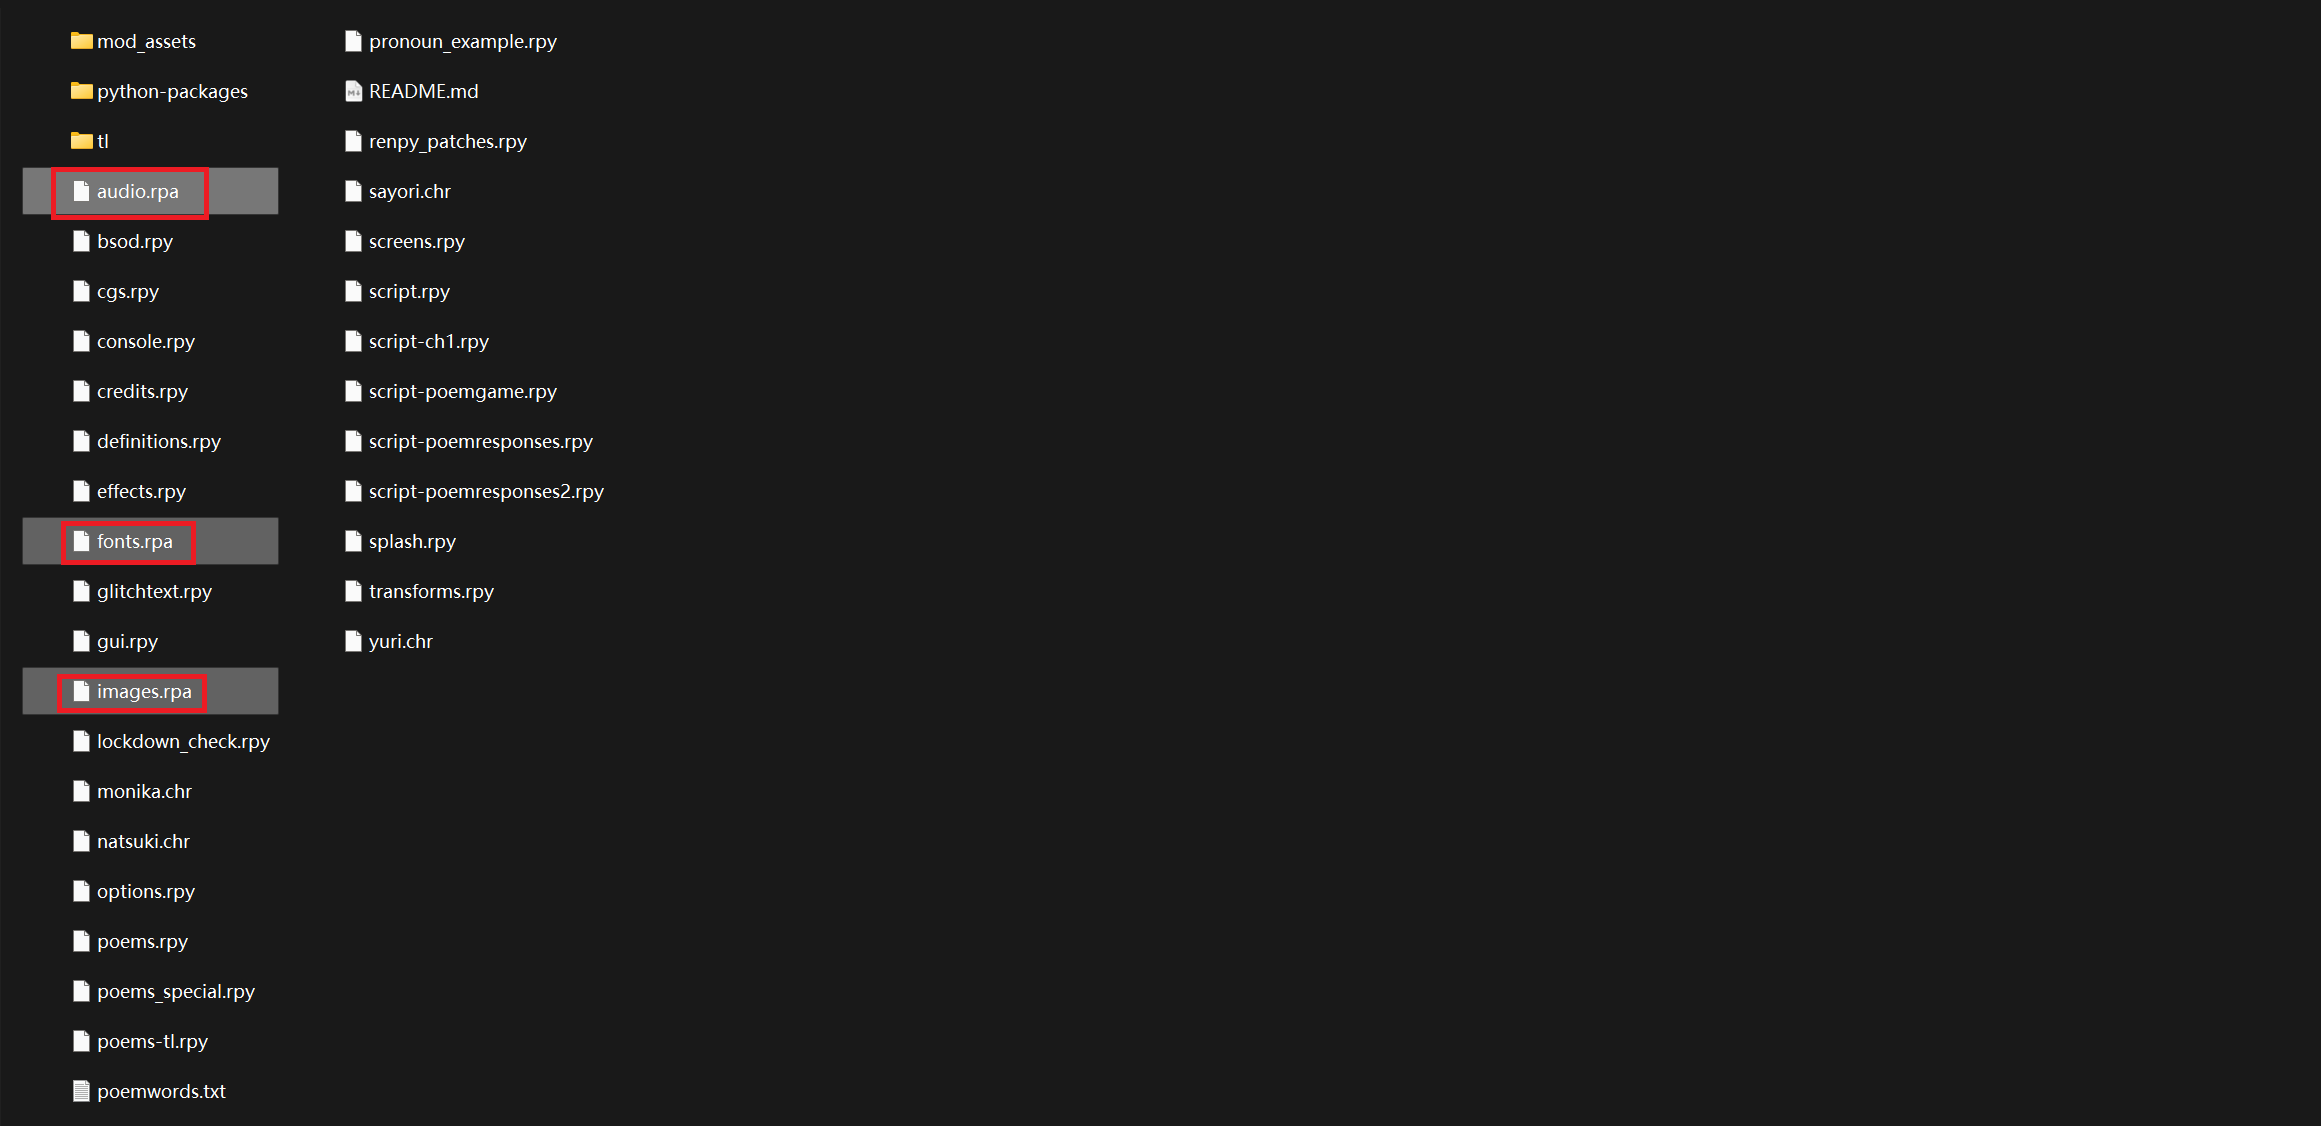
\includegraphics[scale=.2]{2.1/2.1.2}
    \caption{项目结构}
    \label{fig:2.1.1.2}
\end{figure}

至此,您就完成了准备工作的第一部分———下载DDLC Mod中文模板并完成配置。

\subsection{配置文本编辑器}
\label{2.1.2}
有了Mod中文模板,我们还需要一个趁手的编辑器。你大可选择记事本,不过Ren'Py SDK也为我们提供了两种文本编辑器:Visual Studio Code和Atom。本书将以Visual Studio Code为例配置文本编辑器。

打开Ren'Py SDK,点击右下角的设置。在一般选项卡中选择文本编辑器,此时点击第一个选项Visual Studio Code。Ren'Py会开始下载Visual Studio Code与Ren'Py插件。耐心等待一段时间后,会返回到设置界面。此时点击返回,点击DDLCModTemplate-Chinese-next,点击编辑选项卡下的“打开项目”会打开Visual Studio Code(如图\ref{fig:2.1.2.1}所示)。

\begin{figure}[htbp]
    \centering
    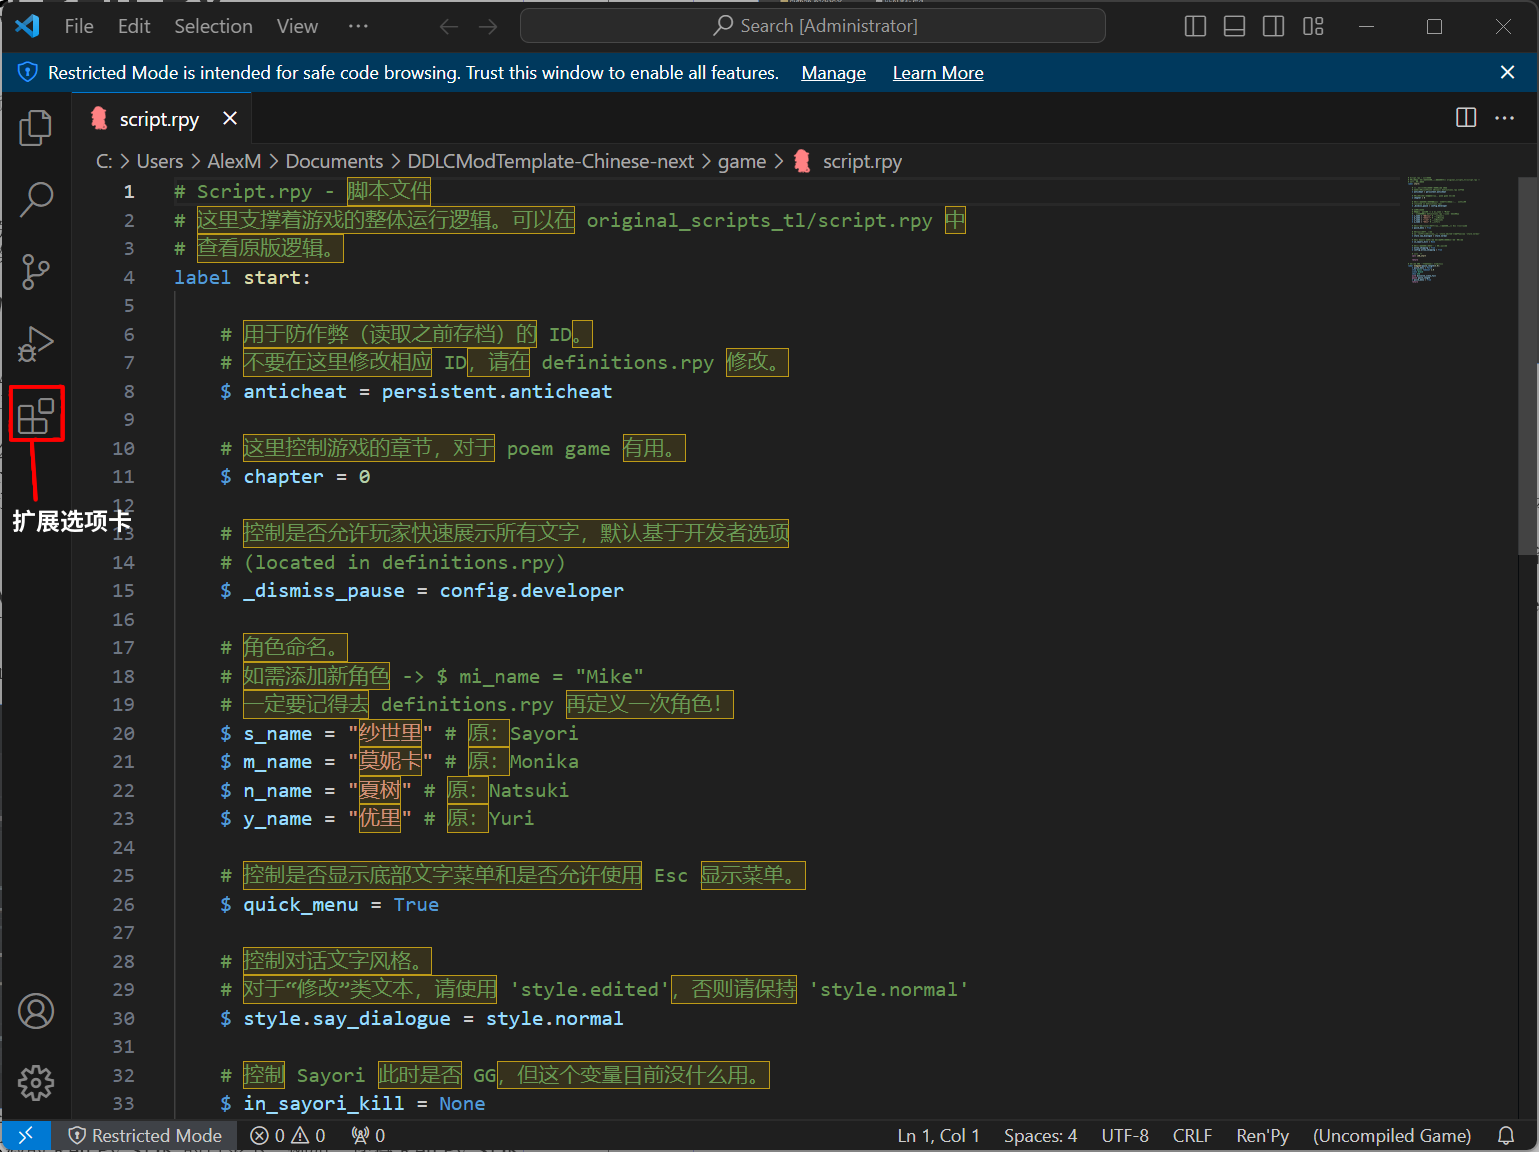
\includegraphics[scale=.4]{2.1/2.1.3}
    \caption{Visual Studio Code}
    \label{fig:2.1.2.1}
\end{figure}

此时点击扩展选项卡,输入Chinese,点击第一个搜索结果中的Install。此时右下角会弹出提示框询问是否切换语言并重启。点击Change Language and Restart。重启后 Visual Studio Code 就会切换成中文。

打开Ren'Py SDK,选中DDLCModTemplate-Chinese-next,点击编辑文件选项卡中的“打开项目”,Ren'Py SDK会自动帮我们打开Visual Studio Code并定位到本项目。

随后,展开左侧资源管理器中的“game”文件夹,打开script-ch1.rpy文件。保留文件第一行,删除其他内容即可。至此,我们就正式完成了开发的准备工作。

\begin{figure}[htbp]
    \centering
    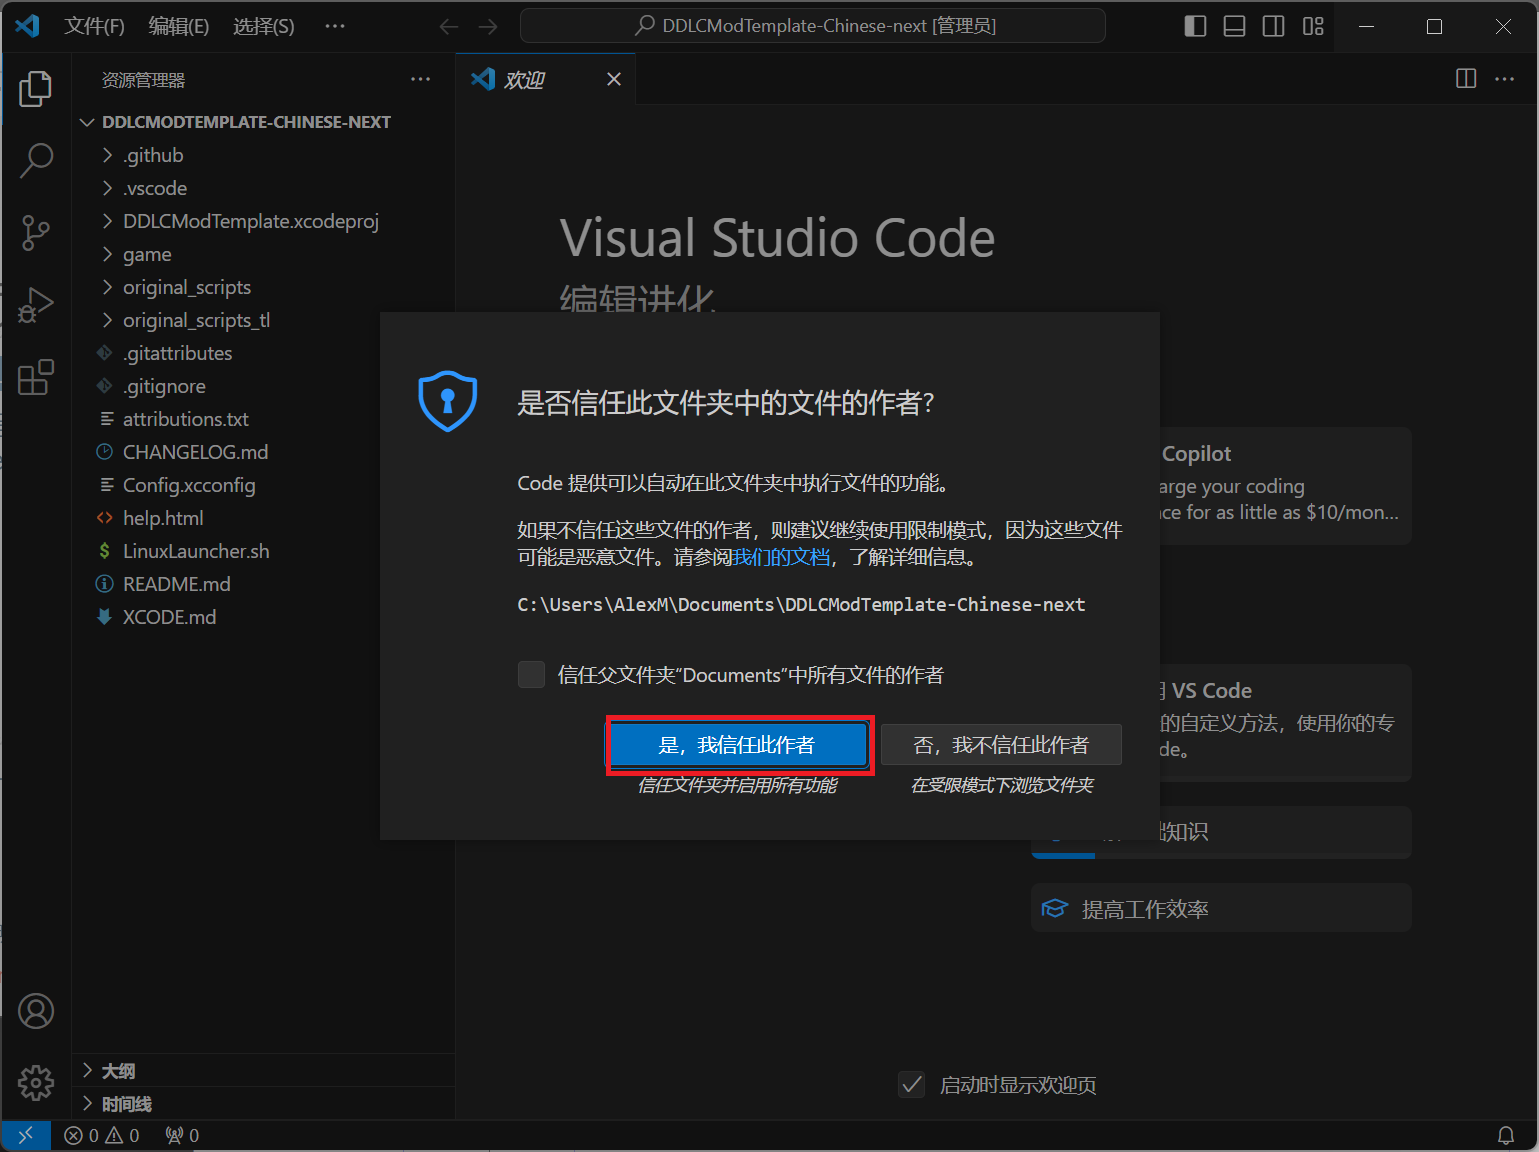
\includegraphics[scale=.4]{2.2/2.2.1}
    \caption{Visual Studio Code}
    \label{fig:2.1.2.2}
\end{figure}
若您打开 Visual Studio Code 时出现如图\ref{fig:2.1.2.2}所示的提示框,请点击“是,我信任此作者”。

\end{document}
